\documentclass[11pt]{article}
\usepackage[T1]{fontenc}
\usepackage{lmodern,amsmath,amssymb,graphicx,xcolor,booktabs,array,enumitem}
\usepackage[letterpaper,margin=0.78in]{geometry}
\usepackage[colorlinks=true,linkcolor=blue,urlcolor=teal]{hyperref}
\usepackage{fancyhdr}
\definecolor{ink}{HTML}{172C3B}
\definecolor{teal}{HTML}{087F82}
\definecolor{blue}{HTML}{265DAB}
\pagestyle{fancy}\fancyhf{}
\fancyhead[L]{\footnotesize OpenAI math: independent illustrated reading editions}
\fancyfoot[C]{\thepage}
\setlength{\headheight}{15pt}
\setlength{\parindent}{0pt}\setlength{\parskip}{7pt}
\setlength{\emergencystretch}{2em}
\hypersetup{pdfauthor={Independent explanatory edition prepared with OpenAI Codex}}
\begin{document}
\begin{center}{\LARGE\bfseries One switch versus a whole group of switches}\par\vspace{12pt}{\large An illustrated reader for sensitivity and block sensitivity}\par\vspace{16pt}Independent reading edition, October 14, 2026\end{center}
\section*{Start here}A Boolean function takes a string of zeros and ones and returns a single zero or one. Sensitivity asks how many individual input bits can reverse that answer at a given input. Block sensitivity allows groups of bits to flip together, but requires the groups to be pairwise disjoint.

The maximum over all inputs is crucial. A function may be completely insensitive at the all-zero string yet very sensitive somewhere else. A proposed global separation must compare the two global quantities, not just convenient values at one input.

The source claims that block sensitivity can grow faster than every constant multiple of sensitivity squared. Its construction keeps many disjoint ways to activate the function while controlling individual-bit changes at all inputs. Nested predicates and a directed tournament organize that control; tracking joint changes of two predicates closes the recursive argument.
\paragraph{Reading prerequisites.} Ordinary arithmetic is enough for the opening examples. Later chapters introduce the specialized vocabulary; checking every original proof requires additional study.\par\textbf{Attribution.} Original manuscript by OpenAI. Added explanations and figures prepared with OpenAI Codex. This is not an official revision or independent theorem validation.\par\href{https://github.com/openai/math/tree/1581d4cbdd69a0faf34b2089614fe2a814316a6a/preprints/A-superquadratic-separation-between-sensitivity-and-block-sensitivity-September-25-2026}{Pinned original manuscript and citation}.\newpage\section*{The source claim, precisely}Theorem 1.1 states that for every $C>0$ there is a nonconstant total Boolean function $f$ with $\operatorname{bs}(f)>Cs(f)^2$. More precisely, the construction yields
\[\frac{\operatorname{bs}(f)}{s(f)^2}\ge\frac{2^d}{4(d+2)^2}\]
for every integer depth $d\ge1$, with sufficiently large construction parameters chosen afterward. The source also amplifies a fixed seed into a power separation with exponent greater than two. This does not contradict the polynomial Sensitivity Conjecture resolved by Huang.\paragraph{How to read this edition.} Each chapter gives one concrete illustration, then explains how it connects to the source. Captions identify toys and original constructions. Source anchors use the original manuscript\textquotesingle s section and page numbering. The expanded PDF places this guide before the complete unchanged original PDF, preserving the original page numbers and bibliography.\subsection*{Your route through the argument}\begin{enumerate}\item A local gap is not a global separation
\item Nested predicates create distinct boundaries
\item A tournament gives every pair of rows one direction
\item Track joint sensitivity alongside ordinary sensitivity
\item An exponential numerator eventually beats a quadratic denominator
\item Composition multiplies disjoint block witnesses
\end{enumerate}\paragraph{Verification scope.} The accompanying code checks the displayed finite examples and preserves original-file hashes. These checks do not replace the analytic, algebraic, asymptotic, or formal proof obligations in the source.\newpage\section*{A local gap is not a global separation}
\begin{center}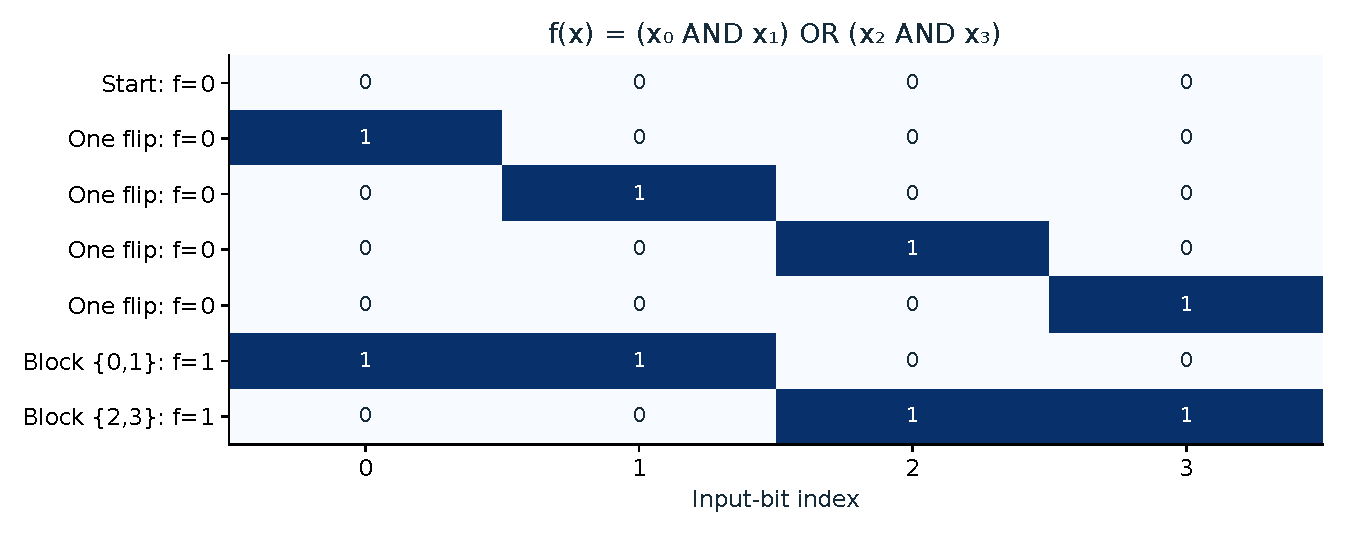
\includegraphics[width=\linewidth,height=2.35in,keepaspectratio]{figures/01-blocks.pdf}\end{center}
{\small\color{teal}\textbf{Figure 1.} For f=(x$_0$ AND x$_1$) OR (x$_2$ AND x$_3$), no single flip changes f at zero, but either of two disjoint pair flips does. Exhaustive checking gives global sensitivity 2 and block sensitivity 2.\par}
At input $0000$, the displayed function outputs zero. Changing one bit cannot make either AND pair true, so $s(f,0000)=0$. Flipping bits $\{0,1\}$ together makes the first pair true; flipping $\{2,3\}$ makes the second pair true. The blocks are disjoint, so $\operatorname{bs}(f,0000)=2$.

That sounds like a large contrast until we ask for the maximum sensitivity across every input. At $1010$, either currently missing partner can activate one of the pairs. Two individual bits are sensitive there. Exhaustive enumeration of all sixteen inputs confirms $s(f)=2$ and $\operatorname{bs}(f)=2$.

The example therefore supplies intuition for cooperative flips but no superquadratic separation. Dividing the local block count by the squared local sensitivity at zero would be meaningless for the theorem.

\paragraph{Disjointness matters.} Blocks cannot share raw input coordinates. Otherwise many overlapping descriptions of the same decisive change would artificially inflate the measure. The source explicitly builds disjoint block families and separately bounds sensitivity at every input, including inputs far from its convenient all-zero witness.
{\footnotesize\color{blue}\textbf{Source anchor:} Section 1 definitions; Section 2.4 disjoint blocks at zero.\par}
\newpage\section*{Nested predicates create distinct boundaries}
\begin{center}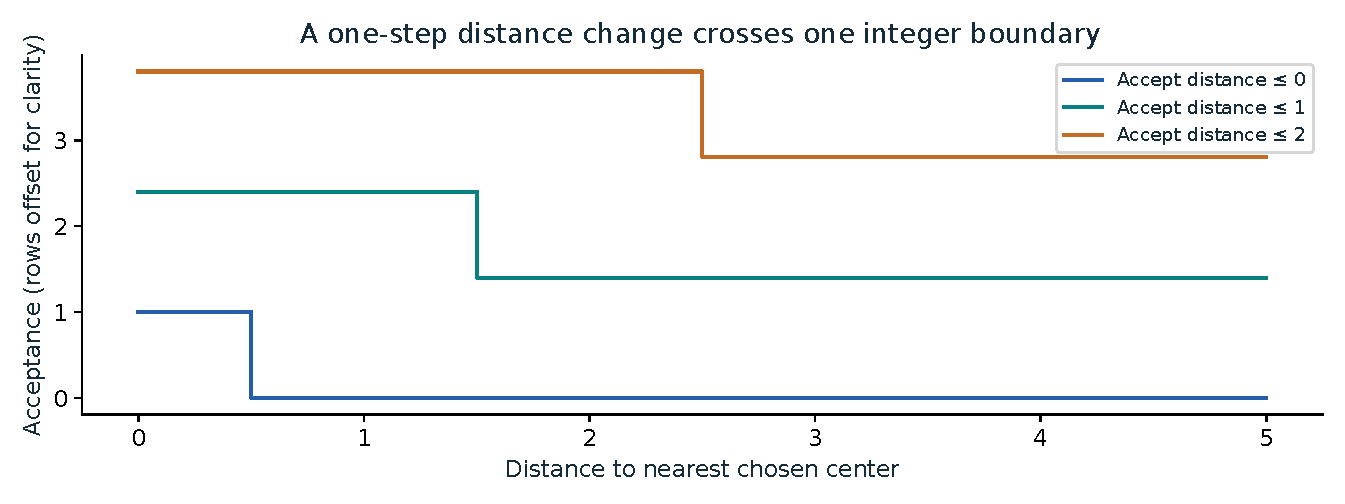
\includegraphics[width=\linewidth,height=2.35in,keepaspectratio]{figures/02-thresholds.pdf}\end{center}
{\small\color{teal}\textbf{Figure 2.} The curves accept distances at most 0, 1, and 2. Their vertical offsets separate the drawing; each predicate itself takes only the values zero and one.\par}
A predicate is a yes-or-no test. A family is nested when every input accepted by a stronger test is also accepted by a weaker one. For example, being within distance zero of a center implies being within distance one, which implies being within distance two.

The source starts with separated centers in a Boolean cube and tests the Hamming distance to the nearest center. Hamming distance counts differing bits. Flipping one raw bit changes that nearest-center distance by at most one: this follows from the triangle inequality, in both directions.

Distinct integer radii give distinct boundaries. A one-unit distance change cannot cross two such boundaries at once, so the initial joint sensitivities vanish. Joint sensitivity counts bits that reverse two distinct predicates simultaneously from the same initial value.

The nesting is in the \emph{predicate index}, not in the input coordinates. These predicates need not be monotone Boolean functions under changing zeros to ones. Confusing those two meanings of monotonicity would invalidate the argument.

The plotted distance axis is a summary of a high-dimensional cube, not its geometric embedding. The source's separated centers are chosen so local sensitivity can also be bounded near each acceptance region.
{\footnotesize\color{blue}\textbf{Source anchor:} Sections 2.1 and 2.3: initial predicates and Lemma 2.2.\par}
\newpage\section*{A tournament gives every pair of rows one direction}
\begin{center}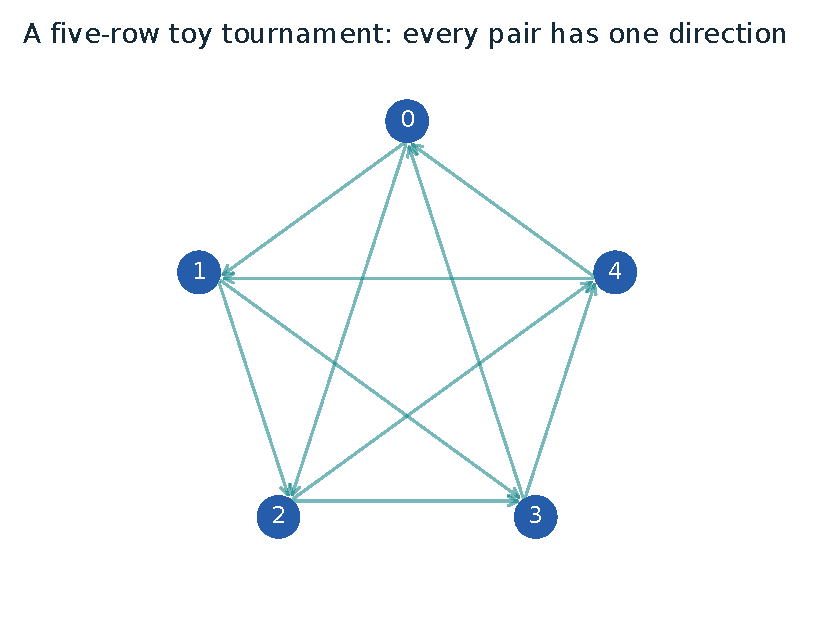
\includegraphics[width=\linewidth,height=2.35in,keepaspectratio]{figures/03-tournament.pdf}\end{center}
{\small\color{teal}\textbf{Figure 3.} This five-row cyclic tournament is a small structural illustration. Each row has two outgoing neighbors. It is not the paper's labeled tournament with k=2M$^2$+1 and M$\ge$3.\par}
A tournament orients every edge of a complete graph: for two different rows, exactly one points toward the other. The picture uses five rows so the entire orientation remains visible. It is an indexing device, not a competition simulation.

In the source, each row contains several child inputs. A clause for row $i$ requires all targets in its own row to accept. For every outgoing edge $i\to j$, it also requires a chosen child in row $j$ to fail a weaker predicate. The edge label specifies which child is tested. The parent accepts if any row clause holds.

All conditions within one clause use distinct children. One raw-bit flip therefore changes at most one condition of that clause. If a rejecting clause becomes true after one flip, it must have had exactly one failing condition beforehand.

For clauses failing only one gate, the induced tournament has outdegree at most one. If there are $m$ such clauses, counting edges gives $m(m-1)/2\le m$, hence $m\le3$. The source combines this observation with a forbidden-label condition that controls the clauses failing one target.

The directed structure limits candidate repairs. Random labels alone are not the entire sensitivity proof.
{\footnotesize\color{blue}\textbf{Source anchor:} Sections 2.2 and 3: recursive clauses and candidate-clause counting.\par}
\newpage\section*{Track joint sensitivity alongside ordinary sensitivity}
\begin{center}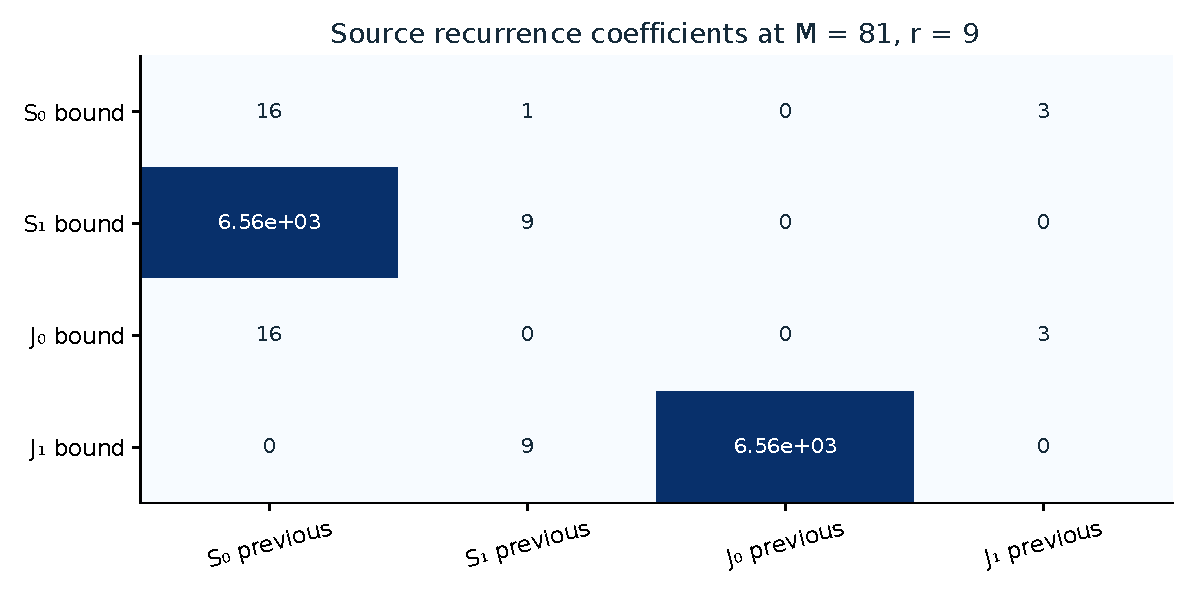
\includegraphics[width=\linewidth,height=2.35in,keepaspectratio]{figures/04-profiles.pdf}\end{center}
{\small\color{teal}\textbf{Figure 4.} The coefficient matrix displays the four inequalities from Proposition 3.1 at M=81 and r=9. Entries multiply previous-level upper bounds; they are not measured sensitivities.\par}
The recursion tracks four quantities: ordinary sensitivity at output zero and one, $S_0,S_1$, and joint sensitivity at output zero and one, $J_0,J_1$. The row labeled $S_0$ reads
\[S_0^{\rm new}\le16S_0^{\rm old}+S_1^{\rm old}+3J_1^{\rm old}.\]
The other rows show the remaining inequalities. Every coefficient is nonnegative, which permits upper bounds to be propagated consistently.

Why introduce $J$? Repairing a gate in a row whose strongest predicate already accepts may require both that strongest predicate and a weaker one to reverse. Counting all such flips by ordinary sensitivity would lose the saving. Joint sensitivity records the more restrictive event.

The source chooses a very large $M$ relative to the intended depth, normalizes the four sequences, and proves a coupled induction. The displayed $M=81$ satisfies the stated size requirement at depth one; it is not a parameter choice for arbitrarily deep recursion.

These are upper-bound recurrences. Equality is neither asserted nor needed. At the final level there is only one parent predicate, so its actual joint profiles vanish even if a generic propagated upper bound remains positive.
{\footnotesize\color{blue}\textbf{Source anchor:} Proposition 3.1 and Section 4 normalization.\par}
\newpage\section*{An exponential numerator eventually beats a quadratic denominator}
\begin{center}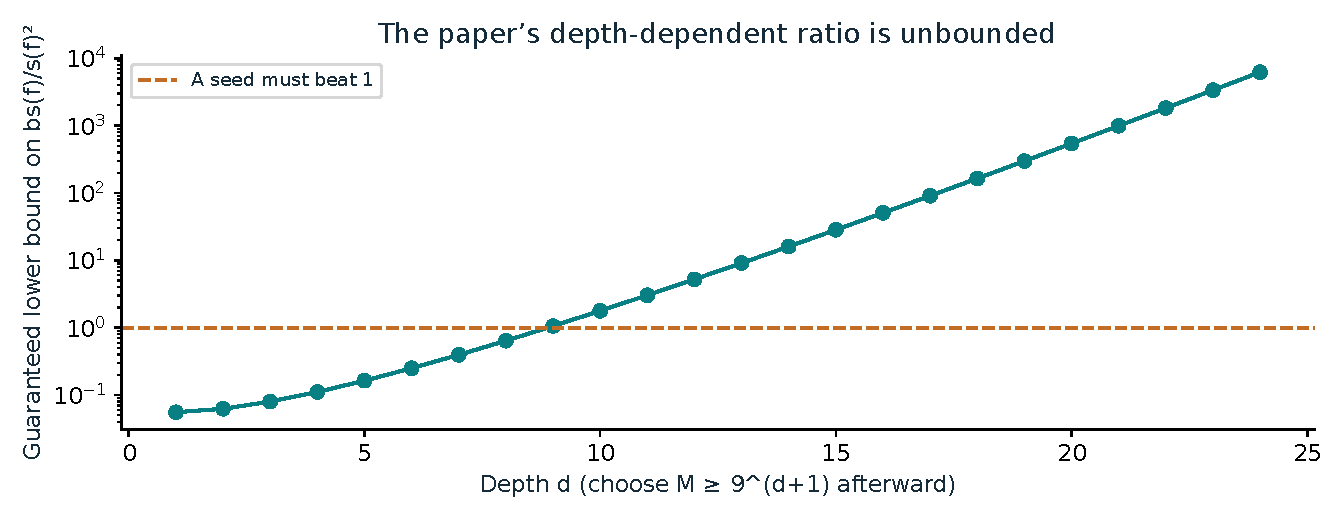
\includegraphics[width=\linewidth,height=2.35in,keepaspectratio]{figures/05-ratio.pdf}\end{center}
{\small\color{teal}\textbf{Figure 5.} The plotted source lower bound 2\textasciicircum{}d/[4(d+2)$^2$] exceeds one at d=9 and tends to infinity. The construction dimension also grows enormously with the required parameter choices.\par}
The source builds many disjoint sensitive blocks at zero and bounds global sensitivity everywhere. After an OR of disjoint copies balances the zero and one cases, its estimates give
\[s(f)\le2(d+2)M^{d+1},\qquad \operatorname{bs}(f,0)\ge M^2(2M^2+1)^d.\]
Dividing yields at least $2^d/[4(d+2)^2]$. The powers of $M$ cancel in this ratio, while the extra factor roughly two per level survives.

At $d=9$, the displayed lower bound is $512/484=128/121>1$. That supplies a depth at which the claimed construction can produce a seed beating the quadratic ratio. It does not provide a small truth table: the source requires $M\ge9^{d+1}$ and uses $n=(d+2)M^2(kr)^d$ raw bits, with $k=2M^2+1$ and $r=\lceil\sqrt M\rceil$.

For an arbitrary proposed constant $C$, first choose a depth making the ratio exceed $C$, then choose the remaining parameters. Reversing that order and holding a small $M$ fixed would not follow the proof.

The chart is a plot of a proven expression within the source argument, not experimental measurements of giant Boolean functions.
{\footnotesize\color{blue}\textbf{Source anchor:} Theorem 1.1 proof, equations (7)-(10).\par}
\newpage\section*{Composition multiplies disjoint block witnesses}
\begin{center}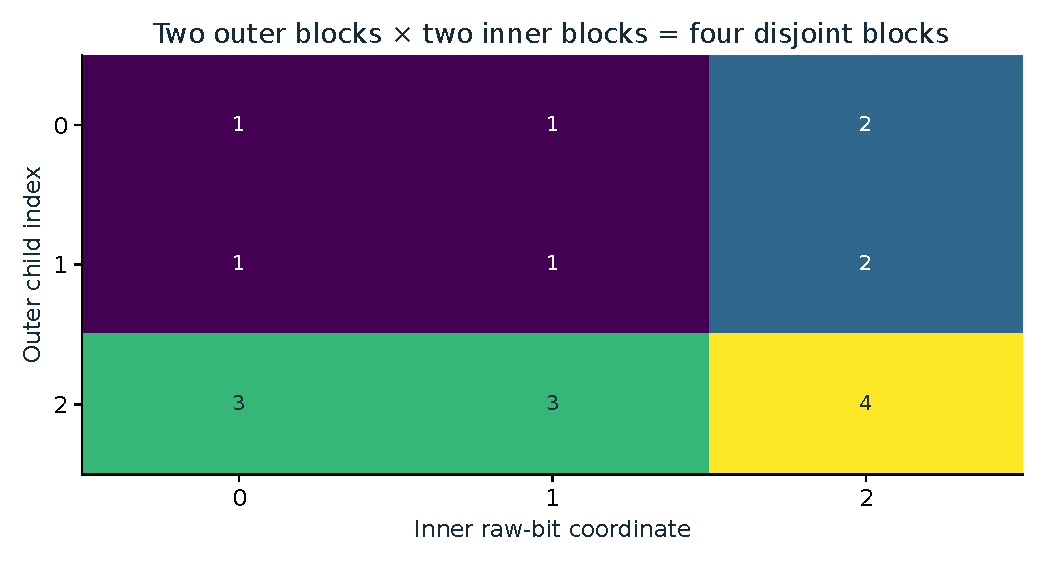
\includegraphics[width=\linewidth,height=2.35in,keepaspectratio]{figures/06-composition.pdf}\end{center}
{\small\color{teal}\textbf{Figure 6.} Each color labels one Cartesian-product block. Two disjoint outer blocks and two disjoint inner blocks give four pairwise disjoint raw-coordinate blocks.\par}
In a composition $f\circ g$, each input bit of $f$ is replaced by the output of a separate copy of $g$. A raw bit can change the final answer only if it changes its child and the corresponding outer coordinate is sensitive. This gives $s(f\circ g)\le s(f)s(g)$.

At the zero input, assuming $g(0)=0$, disjoint sensitive blocks combine by Cartesian products. If $C_i$ is a block of outer child indices and $D_j$ a block of raw positions within a child, use $C_i\times D_j$. Distinct pairs $(i,j)$ remain disjoint. Flipping that set changes exactly the children in $C_i$, triggering the outer witness.

The colored grid makes this disjointness visible. It is a coordinate bookkeeping example; the block shapes are not extracted from a gigantic seed.

If one fixed seed has $b=\operatorname{bs}(f,0)>s(f)^2$ and $f(0)=0$, repeated composition gives block sensitivity at least $b^m$ and sensitivity at most $s(f)^m$. Thus the exponent $\alpha=\log b/\log s(f)$ exceeds two. This is how a strict finite ratio becomes an unbounded family with a fixed power separation.

The construction of a suitable seed remains indispensable; composition cannot manufacture the strict inequality from our introductory four-bit toy.
{\footnotesize\color{blue}\textbf{Source anchor:} Lemma 4.2 and Corollary 4.3.\par}
\newpage\section*{A vocabulary you can return to}
\paragraph{Total Boolean function}A zero-or-one output defined on every binary input of its fixed length.
\paragraph{Sensitivity at x}Number of individual bits that reverse the value at x.
\paragraph{Block sensitivity}Maximum number of disjoint nonempty flip sets that each reverse the value.
\paragraph{Joint sensitivity}Bits that reverse two distinct predicates simultaneously.
\paragraph{Tournament}An orientation of every pair of distinct vertices.
\paragraph{Composition}Replace each outer input bit by an independent child function output.
\section*{What this edition checks}The four-bit toy is exhaustively checked at every input, including a disjoint-block search. The recurrence coefficients and displayed depth ratio are checked arithmetically. This is not a reconstruction or exhaustive evaluation of the source's huge seed, nor an independent audit of its arbitrary-input recurrence proof. The source's attribution to earlier work, including Meiburg's tournament architecture, remains in the reproduced manuscript.
\paragraph{A useful self-test.} Explain what each plotted quantity counts, which examples are illustrative, and where the source needs a statement for every input or every sufficiently large size. If a picture seems to establish the full theorem by itself, revisit its caption and source anchor.\paragraph{Sources and reuse.}\href{https://github.com/openai/math/tree/1581d4cbdd69a0faf34b2089614fe2a814316a6a/preprints/A-superquadratic-separation-between-sensitivity-and-block-sensitivity-September-25-2026}{A superquadratic separation between sensitivity and block sensitivity}, OpenAI. Original bibliography and manuscript-specific citation are included with the source. Source snapshot: \texttt{1581d4cbdd69}. This derivative is distributed under Apache-2.0 with the original attribution; see the repository LICENSE and NOTICE.\end{document}